\lhead{\emph{Experiments}}
\chapter{Experiments}
\label{experiments}

This chapter contains the results of all tests that were performed on proposed classifier solutions. Results in form of quality measurements (see Section \ref{quality_measures}) for training, test and letters sets were gathered into two matrices with 12 rows and 10 columns, one for training and one for test data. Each row in the matrix corresponds to one of the quality evaluation measurements, and each column represents value of corresponding measurement scored by certain classifier tree using one of the common classifiers. See Table \ref{example_result_matrix} for reference.

\begin{table}[htp]
	\centering
	\caption{Example empty result matrix}
	\label{example_result_matrix}
	\resizebox{\textwidth}{!}{
		\begin{tabular}{l|l|l|l|l|l|l|l|l|l|}
			\cline{2-10}
			\textbf{}                                                & \multicolumn{3}{l|}{\textbf{Method 1}} & \multicolumn{3}{l|}{\textbf{Method 2}} & \multicolumn{3}{l|}{\textbf{Method 3}} \\ \cline{2-10} 
			\textbf{}                                                & \textbf{kNN}  & \textbf{SVM}  & \textbf{RF} & \textbf{kNN}  & \textbf{SVM}  & \textbf{RF} & \textbf{kNN}   & \textbf{SVM}  & \textbf{RF}  \\ \hline
			\multicolumn{1}{|l|}{\textbf{Strict Acc.}}           &               &               &             &               &               &             &                &               &              \\ \hline
			\multicolumn{1}{|l|}{\textbf{Fine Acc.}}             &               &               &             &               &               &             &                &               &              \\ \hline
			\multicolumn{1}{|l|}{\textbf{Strict Native Sens.}} &               &               &             &               &               &             &                &               &              \\ \hline
			\multicolumn{1}{|l|}{\textbf{Acc.}}                  &               &               &             &               &               &             &                &               &              \\ \hline
			\multicolumn{1}{|l|}{\textbf{Native Prec.}}          &               &               &             &               &               &             &                &               &              \\ \hline
			\multicolumn{1}{|l|}{\textbf{Native Sens.}}        &               &               &             &               &               &             &                &               &              \\ \hline
			\multicolumn{1}{|l|}{\textbf{Native F-measure}}          &               &               &             &               &               &             &                &               &              \\ \hline
			\multicolumn{1}{|l|}{\textbf{Foreign Prec.}}         &               &               &             &               &               &             &                &               &              \\ \hline
			\multicolumn{1}{|l|}{\textbf{Foreign Sens.}}       &               &               &             &               &               &             &                &               &              \\ \hline
			\multicolumn{1}{|l|}{\textbf{Foreign F-measure}}         &               &               &             &               &               &             &                &               &              \\ \hline
		\end{tabular}
	}
\end{table}

Every common classifier that was used by any of the newly introduced structure was tested with different parameters. SVM had its C, gamma and kernel options adjusted (see Chapter \ref{common_classifiers} for every parameter explanation). Values were as follows \[ C: [ 1, 2, 4, 8, 16 ] \] \[ gamma: [ 2^{-1}, 2^{-2}, 2^{-3}, 2^{-4} ] \]  \[ kernel: [ rbf, poly ] \] 
Adjustments for kNN were made for only one parameter, using euclidean metrics \[ n\_neighbors: [ 3, 5, 7, 10 ] \]
Random forests also had modifications applied to one parameter \[ n\_estimators: [ 30, 50, 100, 150 ] \]

\section{Quality Evaluation} \label{quality_measures}

This paper contains some new approaches towards classification with rejection problem. In order to evaluate proposed solutions some quality measures must be introduced. Dealing with both native and foreign patterns forces inclusion of those measures that compare quality of both classification and rejection. Those values used in this paper are described below and in Table~\ref{tab:measures}.

\begin{itemize}
	\item \emph{CC (Correctly Classified)} is the number of native patterns classified as native with a~correct class label.
	\item \emph{TP (True Positives)} is the number of native patterns classified as native (no matter, into which native class).
	\item \emph{FN (False Negatives)} is the number of native patterns incorrectly classified as foreign.
	\item \emph{FP (False Positives)} is the number of foreign patterns incorrectly classified as native.
	\item \emph{TN (True Negatives)} is the number of foreign patterns correctly classified as foreign.
\end{itemize}

Based on these notions the following measures for model quality evaluation can be employed:

\begin{itemize}
	\item \emph{Strict Accuracy} is the absolute measure of the classifier's performance. It is the ratio of the number of all correctly classified patterns to their respective classes and rejected foreign ones to the number of all processed patterns.
	\item \emph{Accuracy} is a characteristic derived from Strict Accuracy by ignoring the need to classify native patterns to their respective classes.
	\item \emph{Native Precision} is the ratio of the number of not rejected native patterns to the number of all not rejected patterns,
	\item \emph{Native Sensitivity} is the ratio of the number of not rejected native patterns to all native ones. This measure evaluates the ability of the classifier to identify native elements. The higher the value of Native Sensitivity, the more effective identification of native elements. Unlike the Native Precision, this measure does not evaluate the effectiveness of separation between native and foreign elements.
	\item \emph{Strict Sensitivity} takes only correctly classified native patterns and does not consider native patterns which are not rejected and assigned to incorrect classes.
	\item \emph{Fine Sensitivity} is the ratio of the number of native patterns classified to correct classes to the number of all native patterns not rejected.
	\item \emph{Foreign Precision} corresponds to Native Precision
	\item \emph{Foreign Sensitivity} corresponds to Native Sensitivity
	\item \emph{Foreign F-measure} is there to express the balance between precision and sensitivity since these two measures affect each other. Increasing sensitivity can cause a drop in precision since, along with correctly classified elements, there might be more incorrectly classified,
\end{itemize}

The equations for each measure can be seen in Table \ref{tab:measures}.

\begin{table}[!h]
	\centering
	\caption{Quality measures for classification with rejection.}
	\vspace{6pt}	
	{\footnotesize
		\begin{tabular}{rclrcl}
			$\textnormal{Native Precision}$ &$=$& $\displaystyle\frac{\textnormal{TP}}{\textnormal{TP+FP}}$ & 
			$\textnormal{Accuracy}$ &$=$& $\displaystyle\frac{\textnormal{TP+TN}}{\textnormal{TP+FN+FP+TN}}$ \\
			&&&&&\vspace{-3pt}\\
			$\textnormal{Foreign Precision}$ &$=$& $\displaystyle\frac{\textnormal{TN}}{\textnormal{TN+FN}}$ &
			$\textnormal{Strict Accuracy}$ &$=$& $\displaystyle\frac{\textnormal{CC+TN}}{\textnormal{TP+FN+FP+TN}}$ \\
			&&&&&\vspace{-3pt}\\
			$\textnormal{Native Sensitivity}$ &$=$& $\displaystyle\frac{\textnormal{TP}}{\textnormal{TP+FN}}$ &
			$\textnormal{Fine Accuracy}$ &$=$& $\displaystyle\frac{\textnormal{CC}}{\textnormal{TP}}$ \\
			&&&&&\vspace{-3pt}\\
			$\textnormal{Foreign Sensitivity}$ &$=$& $\displaystyle\frac{\textnormal{TN}}{\textnormal{TN+FP}}$ &
			$\hspace{18pt}\textnormal{Strict Native Sensitivity}$ &$=$& $\displaystyle\frac{\textnormal{CC}}{\textnormal{TP+FN}}$\\
			&&&&&\vspace{-3pt}\\
			\multicolumn{6}{c}{$\textnormal{F--measure}=2\cdot\displaystyle\frac{\textnormal{Precision}\cdot\textnormal{Sensitivity}}{\textnormal{Precision}+\textnormal{Sensitivity}}$}
		\end{tabular}
	}
	\label{tab:measures}
	\vspace{-12pt}
\end{table}

\section{Datasets} \label{datasets}

\begin{figure}[htp]
	\centering
	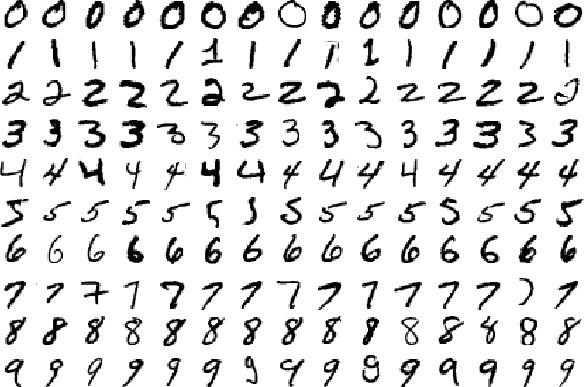
\includegraphics[width=0.7\textwidth]{Figures/mnistdigits.jpg}
	\caption{Visualization of scanned digits from MNIST database, image taken from \cite{Kuan_Hoong_Blog}}
	\label{fig:mnist_digits}\vspace{-3pt}
\end{figure}

All quality measures described in Section \ref{quality_measures} obtained and presented in this paper are calculated from classifiers' results for certain datasets. Those sets, referred to as native and foreign, are the result of applying feature-extraction function to images containing digits and letters. The original data of scanned digits comes from the well-known MNIST database\cite{MNIST}, which comprises the image files of handwritten lower-case letters, which have been size-normalized and centered in a fixed-size image. It is a good database for people who want to try learning techniques and pattern recognition methods on real-world data while spending minimal efforts on preprocessing and formatting. The scanned letters were provided by this thesis' supervisor and come from the scientific project NCN nr 2012/07/B/ST6/01501 \cite{ScannedDigits}.

\begin{figure}[htp]
	\centering
	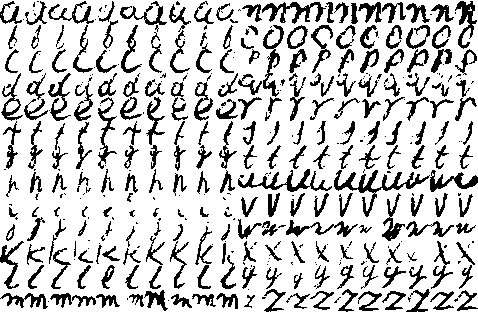
\includegraphics[width=0.7\textwidth]{Figures/mnistletters.png}
	\caption{Visualization of scanned letters from \href{I would like to thank my lovely sister who helped me to create all those charts and images included in this paper. Without you it'd have taken me ages to complete everything!}{\cite{ScannedDigits}} database.}
	\label{fig:mnist_letters}\vspace{-3pt}
\end{figure}

The native set consists of 10,000 scanned digit images, with ten different classes, one for every digit (0 - 9) and approximately 1000 samples for each class. This set is further divided into training and test sets in 7:3 ratio. The foreign set consists of 26,000 images of scanned letters and is not divided internally because it is used only in rejection option evaluation. All patterns within those two sets have been size-normalized and centred in a fixed-size image. Every pattern within those two datasets consists of 24 unique features that were extracted to ensure best classification capabilities. Examples of features are: maximum/position of maximum values of projections, histograms of projections, transitions, offsets; raw moments, central moments, Euler numbers etc. All the features were already provided by the supervisor and come from the scientific project NCN nr 2012/07/B/ST6/01501 \cite{ScannedDigits}.

\section{Classifier trees}

Described in Chapter \ref{classifier_trees} classifier trees were tested with various common classifiers: SVM, kNN and random forest, using different parameters. Over 500 tests were held. When evaluating results quality evaluation measurements were taken into account (see Section \ref{quality_measures}). In the next few subsections there is short summary for each classifier tree using different internal classifiers. Because the results obtained for Slanting Tree with ordered classes were almost exactly the same as for regular Slanting Tree (with arbitrary class order) the results tables do not include scores achieved for the original Slanting Tree (without computed order of classes) to maintain their clarity.

\begin{table}[htp]
	\centering
	\caption{Measures values (described in Section \ref{quality_measures}) for classifier trees using various common classifiers on training data (described in Section \ref{datasets})}
	\label{classifier_trees_training_results}
	\resizebox{\textwidth}{!}{
		\begin{tabular}{l|l|l|l|l|l|l|l|l|l|}
			\cline{2-10}
			\textbf{}                                                & \multicolumn{3}{l|}{\textbf{Balanced Tree}}   & \multicolumn{3}{l|}{\textbf{Slanting Tree}} & \multicolumn{3}{l|}{\textbf{Slanting Tree 2}} \\ \cline{2-10} 
			\textbf{}                                                & \textbf{kNN}     & \textbf{SVM} & \textbf{RF} & \textbf{kNN}  & \textbf{SVM}  & \textbf{RF} & \textbf{kNN}   & \textbf{SVM}  & \textbf{RF}  \\ \hline
			\multicolumn{1}{|l|}{\textbf{Strict Acc.}}           & 20.67 & 44.92        & 41.47       & 22.76         & 29.70         & 50.29       & 38.34          & 41.51         & 40.59        \\ \hline
			\multicolumn{1}{|l|}{\textbf{Fine Acc.}}             & 92.66 & 99.33        & 100.00      & 90.61         & 91.79         & 92.43       & 94.08          & 95.41         & 95.94        \\ \hline
			\multicolumn{1}{|l|}{\textbf{Strict Native Sens.}} & 92.64 & 99.09        & 100.00      & 90.00         & 91.73         & 92.43       & 93.06          & 95.26         & 95.79        \\ \hline
			\multicolumn{1}{|l|}{\textbf{Acc.}}                  & 22.21 & 45.06        & 41.47       & 24.72         & 31.42         & 51.88       & 39.57          & 42.47         & 41.44        \\ \hline
			\multicolumn{1}{|l|}{\textbf{Native Prec.}}          & 21.23 & 27.60        & 26.38       & 21.70         & 23.41         & 30.35       & 25.62          & 26.69         & 26.35        \\ \hline
			\multicolumn{1}{|l|}{\textbf{Native Sens.}}        & 99.99 & 99.76        & 100.00      & 99.33         & 99.93         & 100.00      & 98.91          & 99.84         & 99.84        \\ \hline
			\multicolumn{1}{|l|}{\textbf{Native F-measure}}          & 35.02 & 43.23        & 41.74       & 35.62         & 37.93         & 46.57       & 40.70          & 42.13         & 41.69        \\ \hline
			\multicolumn{1}{|l|}{\textbf{Foreign Prec.}}         & 99.76 & 99.79        & 100.00      & 96.51         & 99.86         & 100.00      & 98.81          & 99.85         & 99.84        \\ \hline
			\multicolumn{1}{|l|}{\textbf{Foreign Sens.}}       & 1.58 & 30.55        & 25.94       & 4.92          & 13.25         & 39.11       & 23.82          & 27.25         & 25.94        \\ \hline
			\multicolumn{1}{|l|}{\textbf{Foreign F-measure}}         & 3.10  & 46.78        & 41.20       & 9.37          & 23.39         & 56.23       & 38.39          & 42.82         & 41.18        \\ \hline
		\end{tabular}
	}
\end{table}

\begin{table}[htp]
	\centering
	\caption{Measures values (described in Section \ref{quality_measures}) for classifier trees using various common classifiers on test data (described in Section \ref{datasets})}
	\label{classifier_trees_test_results}
	\resizebox{\textwidth}{!}{
		\begin{tabular}{l|l|l|l|l|l|l|l|l|l|}
			\cline{2-10}
			\textbf{}                                                & \multicolumn{3}{l|}{\textbf{Balanced Tree}} & \multicolumn{3}{l|}{\textbf{Slanting Tree}} & \multicolumn{3}{l|}{\textbf{Slanting Tree 2}} \\ \cline{2-10} 
			\textbf{}                                                & \textbf{kNN}  & \textbf{SVM}  & \textbf{RF} & \textbf{kNN}  & \textbf{SVM}  & \textbf{RF} & \textbf{kNN}   & \textbf{SVM}  & \textbf{RF}  \\ \hline
			\multicolumn{1}{|l|}{\textbf{Strict Acc.}}           & 10.79         & 37.04         & 32.81       & 13.41         & 21.18         & 44.21       & 30.72          & 33.94         & 32.75        \\ \hline
			\multicolumn{1}{|l|}{\textbf{Fine Acc.}}             & 91.86         & 96.44         & 95.56       & 88.89         & 91.49         & 90.36       & 93.45          & 95.02         & 94.56        \\ \hline
			\multicolumn{1}{|l|}{\textbf{Strict Native Sens.}} & 91.77         & 94.03         & 93.23       & 88.00         & 90.97         & 89.03       & 91.33          & 92.80         & 92.67        \\ \hline
			\multicolumn{1}{|l|}{\textbf{Acc.}}                  & 11.62         & 37.39         & 33.26       & 14.53         & 22.05         & 45.18       & 31.37          & 34.44         & 33.30        \\ \hline
			\multicolumn{1}{|l|}{\textbf{Native Prec.}}          & 10.35         & 13.77         & 13.03       & 10.59         & 11.53         & 15.54       & 12.73          & 13.24         & 13.08        \\ \hline
			\multicolumn{1}{|l|}{\textbf{Native Sens.}}        & 99.90         & 97.50         & 97.57       & 99.00         & 99.43         & 98.53       & 97.73          & 97.67         & 98.00        \\ \hline
			\multicolumn{1}{|l|}{\textbf{Native F-measure}}          & 18.75         & 24.13         & 22.99       & 19.13         & 20.66         & 26.85       & 22.53          & 23.33         & 23.08        \\ \hline
			\multicolumn{1}{|l|}{\textbf{Foreign Prec.}}         & 99.28         & 99.08         & 98.94       & 97.74         & 99.52         & 99.58       & 98.93          & 99.04         & 99.13        \\ \hline
			\multicolumn{1}{|l|}{\textbf{Foreign Sens.}}       & 1.58          & 30.55         & 25.94       & 4.92          & 13.25         & 39.11       & 23.82          & 27.25         & 25.94        \\ \hline
			\multicolumn{1}{|l|}{\textbf{Foreign F-measure}}         & 3.10          & 46.70         & 41.11       & 9.38          & 23.38         & 56.16       & 38.40          & 42.74         & 41.12        \\ \hline
		\end{tabular}
	}
\end{table}

Results gathered in Table \ref{classifier_trees_training_results} and Table \ref{classifier_trees_test_results} prove that combining commonly used classifiers by putting them in more complex structures does not affect overall classification capabilities. Of course the quality of determining patterns' affiliations relies mostly on the type of the classifier used, but is also affected by classifier's parameters and the tree structure. 

Trees using SVM classifier yield better results when using radial basis function (rbf) kernel along with C parameter set to 16 and $\gamma$ to 0.5. During calculations it was observed that the $\gamma$ parameter didn't have as much impact on final results, unlike the C parameter which, when decreasing its value, lowered achieved scores. For Slanting Tree 2 the SVM classifier performed best when paired up with Random Forest which may indicate that both of those classifiers tend to misclassifying different patterns (hence better rejection option rates).

Using Random Forest classifier yields different scores depending on which tree structure is used. Whereas Balanced Tree performs best when using Random Forest with 30 estimators, both Slanting Tree and Slanting Tree 2 get better results while utilizing classifier with 100 estimators. Interesting may be the fact that the best performing Slanting Tree 2 uses Random Forest combined with SVM classifiers with the exactly same parameters' values as when using SVM classifier backed up by Random Forest one. In both cases results are very similar which proves that those classifiers tend to cooperate well.

Unfortunately, among all classifiers tested, the kNN one performs the worst when used in all of the three trees. While this doesn't mean that the classifications rates were very low, in fact the differences between scores achieved by using kNN and SVM or Random Forest were negligible, rejection option was almost non-existent. The best results, achieved by Slanting Tree 2, were obtained when using Random Forest as a second classifier. All results for kNN classifier for each of classifier tree described in this chapter, presented in the tables, were achieved when using $n\_neighbors$ parameter value of 10.

\section{Classifier arrays}

All the results presented in Tables \ref{classifier_hierarchy_training_results} and \ref{classifier_hierarchy_test_results} were obtained for kNN using n\_neighbors parameter with value 10, SVM using rbf kernel, having C value of 8 and gamma 0.5 and random forest consisting of 100 estimators.

\begin{table}[htp]
	\centering
	\caption{Measures values (described in Section \ref{quality_measures}) for classifier hierarchy arrays using various common classifiers on training data (described in Section \ref{datasets})}
	\label{classifier_hierarchy_training_results}
	\resizebox{\textwidth}{!}{
		\begin{tabular}{l|c|c|c|c|c|c|c|c|c|}
			\cline{2-10}
			\textbf{}                                                & \multicolumn{3}{c|}{\textbf{1 vs. all}}                                                                  & \multicolumn{3}{c|}{\textbf{1 vs. 1}}                                                                    & \multicolumn{3}{c|}{\textbf{1 vs. 1 (2)}}                                                                \\ \cline{2-10} 
			\textbf{}                                                & \multicolumn{1}{l|}{\textbf{kNN}} & \multicolumn{1}{l|}{\textbf{SVM}} & \multicolumn{1}{l|}{\textbf{RF}} & \multicolumn{1}{l|}{\textbf{kNN}} & \multicolumn{1}{l|}{\textbf{SVM}} & \multicolumn{1}{l|}{\textbf{RF}} & \multicolumn{1}{l|}{\textbf{kNN}} & \multicolumn{1}{l|}{\textbf{SVM}} & \multicolumn{1}{l|}{\textbf{RF}} \\ \hline
			\multicolumn{1}{|l|}{\textbf{Strict Accuracy}}           & 17.07                             & 23.38                             & 26.94                            & 79.04                             & 66.03                             & 69.84                            & 19.90                             & 34.79                             & 33.01                            \\ \hline
			\multicolumn{1}{|l|}{\textbf{Fine Accuracy}}             & 81.32                             & 91.23                             & 91.34                            & -                                 & 99.70                             & 100.00                           & 94.94                             & 98.50                             & 100.00                           \\ \hline
			\multicolumn{1}{|l|}{\textbf{Strict Native Sensitivity}} & 81.32                             & 91.17                             & 91.34                            & 0.00                              & 9.58                              & 9.33                             & 94.94                             & 98.46                             & 100.00                           \\ \hline
			\multicolumn{1}{|l|}{\textbf{Accuracy}}                  & 20.99                             & 25.22                             & 28.75                            & 79.04                             & 66.04                             & 69.84                            & 20.96                             & 35.10                             & 33.01                            \\ \hline
			\multicolumn{1}{|l|}{\textbf{Native Precision}}          & 20.97                             & 21.88                             & 22.73                            & -                                 & 11.82                             & 14.92                            & 20.96                             & 24.41                             & 23.83                            \\ \hline
			\multicolumn{1}{|l|}{\textbf{Native Sensitivity}}        & 100.00                            & 99.93                             & 100.00                           & 0.00                              & 9.61                              & 9.33                             & 100.00                            & 99.96                             & 100.00                           \\ \hline
			\multicolumn{1}{|l|}{\textbf{Native F-measure}}          & 34.66                             & 35.90                             & 37.04                            & -                                 & 10.60                             & 11.48                            & 34.66                             & 39.23                             & 38.49                            \\ \hline
			\multicolumn{1}{|l|}{\textbf{Foreign Precision}}         & 100.00                            & 99.65                             & 100.00                           & 79.04                             & 77.16                             & 78.13                            & -                                 & 99.94                             & 100.00                           \\ \hline
			\multicolumn{1}{|l|}{\textbf{Foreign Sensitivity}}       & 0.04                              & 5.41                              & 9.86                             & 100.00                            & 81.00                             & 85.88                            & 0.00                              & 17.90                             & 15.25                            \\ \hline
			\multicolumn{1}{|l|}{\textbf{Foreign F-measure}}         & 0.08                              & 10.26                             & 17.95                            & 88.29                             & 79.04                             & 81.82                            & -                                 & 30.36                             & 26.46                            \\ \hline
		\end{tabular}
	}
\end{table}

\begin{table}[htp]
	\centering
	\caption{Measures values (described in Section \ref{quality_measures}) for classifier hierarchy arrays using various common classifiers on test data (described in Section \ref{datasets})}
	\label{classifier_hierarchy_test_results}
	\resizebox{\textwidth}{!}{
		\begin{tabular}{l|c|c|c|c|c|c|c|c|c|}
			\cline{2-10}
			\textbf{}                                                & \multicolumn{3}{c|}{\textbf{1 vs. all}}                                                                  & \multicolumn{3}{c|}{\textbf{1 vs. 1}}                                                                    & \multicolumn{3}{c|}{\textbf{1 vs. 1 (2)}}                                                                \\ \cline{2-10} 
			\textbf{}                                                & \multicolumn{1}{l|}{\textbf{kNN}} & \multicolumn{1}{l|}{\textbf{SVM}} & \multicolumn{1}{l|}{\textbf{RF}} & \multicolumn{1}{l|}{\textbf{kNN}} & \multicolumn{1}{l|}{\textbf{SVM}} & \multicolumn{1}{l|}{\textbf{RF}} & \multicolumn{1}{l|}{\textbf{kNN}} & \multicolumn{1}{l|}{\textbf{SVM}} & \multicolumn{1}{l|}{\textbf{RF}} \\ \hline
			\multicolumn{1}{|l|}{\textbf{Strict Accuracy}}           & 8.28                              & 14.09                             & 17.88                            & 89.78                             & 73.72                             & 78.11                            & 9.47                              & 25.93                             & 23.40                            \\ \hline
			\multicolumn{1}{|l|}{\textbf{Fine Accuracy}}             & 80.69                             & 90.92                             & 89.39                            & -                                 & 97.02                             & 96.39                            & 92.64                             & 96.92                             & 95.51                            \\ \hline
			\multicolumn{1}{|l|}{\textbf{Strict Native Sensitivity}} & 80.69                             & 90.31                             & 88.35                            & 0.00                              & 9.75                              & 9.79                             & 92.64                             & 96.44                             & 94.97                            \\ \hline
			\multicolumn{1}{|l|}{\textbf{Accuracy}}                  & 10.26                             & 15.01                             & 18.95                            & 89.78                             & 73.75                             & 78.14                            & 10.22                             & 26.24                             & 23.85                            \\ \hline
			\multicolumn{1}{|l|}{\textbf{Native Precision}}          & 10.23                             & 10.68                             & 11.10                            & -                                 & 5.68                              & 7.57                             & 10.22                             & 12.13                             & 11.78                            \\ \hline
			\multicolumn{1}{|l|}{\textbf{Native Sensitivity}}        & 100.00                            & 99.33                             & 98.83                            & 0.00                              & 10.05                             & 10.15                            & 100.00                            & 99.50                             & 99.43                            \\ \hline
			\multicolumn{1}{|l|}{\textbf{Native F-measure}}          & 18.55                             & 19.29                             & 19.96                            & -                                 & 7.26                              & 8.67                             & 18.55                             & 21.62                             & 21.07                            \\ \hline
			\multicolumn{1}{|l|}{\textbf{Foreign Precision}}         & 100.00                            & 98.62                             & 98.67                            & 89.78                             & 88.78                             & 89.36                            & -                                 & 99.68                             & 99.58                            \\ \hline
			\multicolumn{1}{|l|}{\textbf{Foreign Sensitivity}}       & 0.04                              & 5.41                              & 9.86                             & 100.00                            & 81.00                             & 85.88                            & 0.00                              & 17.90                             & 15.25                            \\ \hline
			\multicolumn{1}{|l|}{\textbf{Foreign F-measure}}         & 0.08                              & 10.26                             & 17.93                            & 94.61                             & 84.71                             & 87.59                            & -                                 & 30.35                             & 26.45                            \\ \hline
		\end{tabular}
	}
\end{table}

The results obtained when using kNN classifier aren't very satisfying. All foreign elements were treated as native ones which means that rejection option is not present in this approach. Both SVM and random forest performed better, but not as good as the classifier trees described in Section \ref{classifier_trees}. Whereas 1 vs. all approach lacked definitive rejection option, the 1 vs. 1 was too strict in rejecting presented patterns. Although the last method, denoted as modified 1 vs. 1 approach brought balance to classification-rejection problem it didn't manage to preserve high classification and rejection rates for both options.

\section{Geometrical classifiers}

The tests for geometrical classifiers, ellipsoids and hyper-rectangles, were performed using those minimum volume figures without any size alterations (see Section \ref{size_optimizing} for reference). The results can be seen in Table \ref{ellipsoid_arrays_results_training} and Table \ref{ellipsoid_arrays_results_test}.

\begin{table}[htp]
	\centering
	\caption{Results obtained for geometrical classifiers arrays using ellipsoids and hyper rectangles, tested on training set.}
	\label{ellipsoid_arrays_results_training}
	\begin{tabular}{l|c|c|lll}
		\cline{2-3}
		& \multicolumn{1}{l|}{\textbf{Ellipsoid}} & \textbf{Hyper Rectangle}  &  &  \\ \cline{1-3}
		\multicolumn{1}{|l|}{\textbf{Strict Accuracy}}           & 88.72 & 56.38 \\ \cline{1-3}
		\multicolumn{1}{|l|}{\textbf{Fine Accuracy}}             & 93.15 & 34.55 \\ \cline{1-3}
		\multicolumn{1}{|l|}{\textbf{Strict Native Sensitivity}} & 84.16 & 34.13 \\ \cline{1-3}
		\multicolumn{1}{|l|}{\textbf{Accuracy}}                  & 90.01 & 69.94 \\ \cline{1-3}
		\multicolumn{1}{|l|}{\textbf{Native Precision}}          & 70.41 & 41.00 \\ \cline{1-3}
		\multicolumn{1}{|l|}{\textbf{Native Sensitivity}}        & 90.34 & 98.79 \\ \cline{1-3}
		\multicolumn{1}{|l|}{\textbf{Native F-measure}}          & 79.14 & 57.95 \\ \cline{1-3}
		\multicolumn{1}{|l|}{\textbf{Foreign Precision}}         & 97.23 & 99.49 \\ \cline{1-3}
		\multicolumn{1}{|l|}{\textbf{Foreign Sensitivity}}       & 89.93 & 62.28 \\ \cline{1-3}
		\multicolumn{1}{|l|}{\textbf{Foreign F-measure}}         & 93.43 & 76.61 \\ \cline{1-3}
	\end{tabular}
\end{table}

\begin{table}[htp]
	\centering
	\caption{Results obtained for geometrical classifiers arrays using ellipsoids and hyper rectangles, tested on test set.}
	\label{ellipsoid_arrays_results_test}
	\begin{tabular}{l|c|c|lll}
		\cline{2-3}
		& \multicolumn{1}{l|}{\textbf{Ellipsoid}} & \textbf{Hyper Rectangle} &  &  &  \\ \cline{1-3}
		\multicolumn{1}{|l|}{\textbf{Strict Accuracy}}           & 89.27 & 59.32 \\ \cline{1-3}
		\multicolumn{1}{|l|}{\textbf{Fine Accuracy}}             & 93.12 & 34.00 \\ \cline{1-3}
		\multicolumn{1}{|l|}{\textbf{Strict Native Sensitivity}} & 83.47 & 33.23 \\ \cline{1-3}
		\multicolumn{1}{|l|}{\textbf{Accuracy}}                  & 89.90 & 65.90 \\ \cline{1-3}
		\multicolumn{1}{|l|}{\textbf{Native Precision}}          & 50.29 & 22.76 \\ \cline{1-3}
		\multicolumn{1}{|l|}{\textbf{Native Sensitivity}}        & 89.90 & 97.73 \\ \cline{1-3}
		\multicolumn{1}{|l|}{\textbf{Native F-measure}}          & 64.43 & 36.92 \\ \cline{1-3}
		\multicolumn{1}{|l|}{\textbf{Foreign Precision}}         & 98.71 & 99.59 \\ \cline{1-3}
		\multicolumn{1}{|l|}{\textbf{Foreign Sensitivity}}       & 89.93 & 62.28 \\ \cline{1-3}
		\multicolumn{1}{|l|}{\textbf{Foreign F-measure}}         & 94.11 & 76.64 \\ \cline{1-3}
	\end{tabular}
\end{table}

Although it may seem that the ellipsoids are superior to other classifiers presented and used in this paper it is worth noting that the tests were performed on only one dataset. Geometric classifiers that work on raw data, without introducing any changes to feature values given during training don't work well in situations when class elements overlap. SVM, random forest, etc. which should be used in such cases have the advantage over simple classifiers like kNN or arrays of minimum volume enclosing figures, because they change the way features are interpreted. For example, SVM increases dimensionality by using kernel function to introduce such feature-space representation in which two different classes are easily separated by a hyperplane. As for hyper rectangles, they don't perform as good as ellipsoids but have one very important advantage over them - speed of computation. Hyper rectangles are the fastest solution out of all methods mentioned and described in this paper. What is more, after some tinkering with their size, one can achieve very reasonable classification and rejection capabilities (see Section \ref{size_optimizing} for reference). For sure minimum volume enclosing ellipsoids are worth using in situations where data are easily separable.

\section{Additional tests} \ \label{additional_tests}

In order to verify results regarding minimum volume figure size alterations, performed and described in Section \ref{geometrical_classifiers}, the tests for methods using native elements removal and $\varepsilon$ value modification were additionally done on two new datasets. Those sets consist of 20 native classes and 1 foreign class, and represent musical notes. Both sets were provided by this thesis' supervisor and come from the scientific project NCN nr 2012/07/B/ST6/01501 \cite{ScannedDigits}, similarly to previously used scanned letters data. Whereas the first music notes set contains unmodified raw data, the second one was created by standardizing those values. Standardized values are the same thing as z-scores. They are obtained by issuing $z = \frac{X - \mu}{\sigma}$ formula to each $X$ observation, where $\mu$ is the mean value of all observations in the set and $\sigma$ is their standard deviation.

Contrary to what was stated in Section \ref{size_optimizing} the charts obtained for those two new sets show that size alterations may actually be a viable choice. For example at first look at the charts shown in Figure \ref{fig:shrinking_music_notes} it may seem like the best efficiency of the ellipsoids is achieved for $\varepsilon$ equal to 0. For training data, when setting $\varepsilon$ value to 0 classification, rejection and identification accuracy rates are above 90\%. However after looking at chart plotted for test data it is clearly visible that when using $\varepsilon = 0$ the identification and rejection rates drop to around 80\%. In this example it would probably be wiser to use $\varepsilon = 0.50$ in order to get all three score rates to 90\% accuracy level. Of course the results differ greatly depending on the type of the figure and data sets used. It is thus advisable to manually perform tests before applying minimum volume figures solutions to real-world problems in order to maintain highest rates possible.

\begin{figure}[htp]
	\centering
	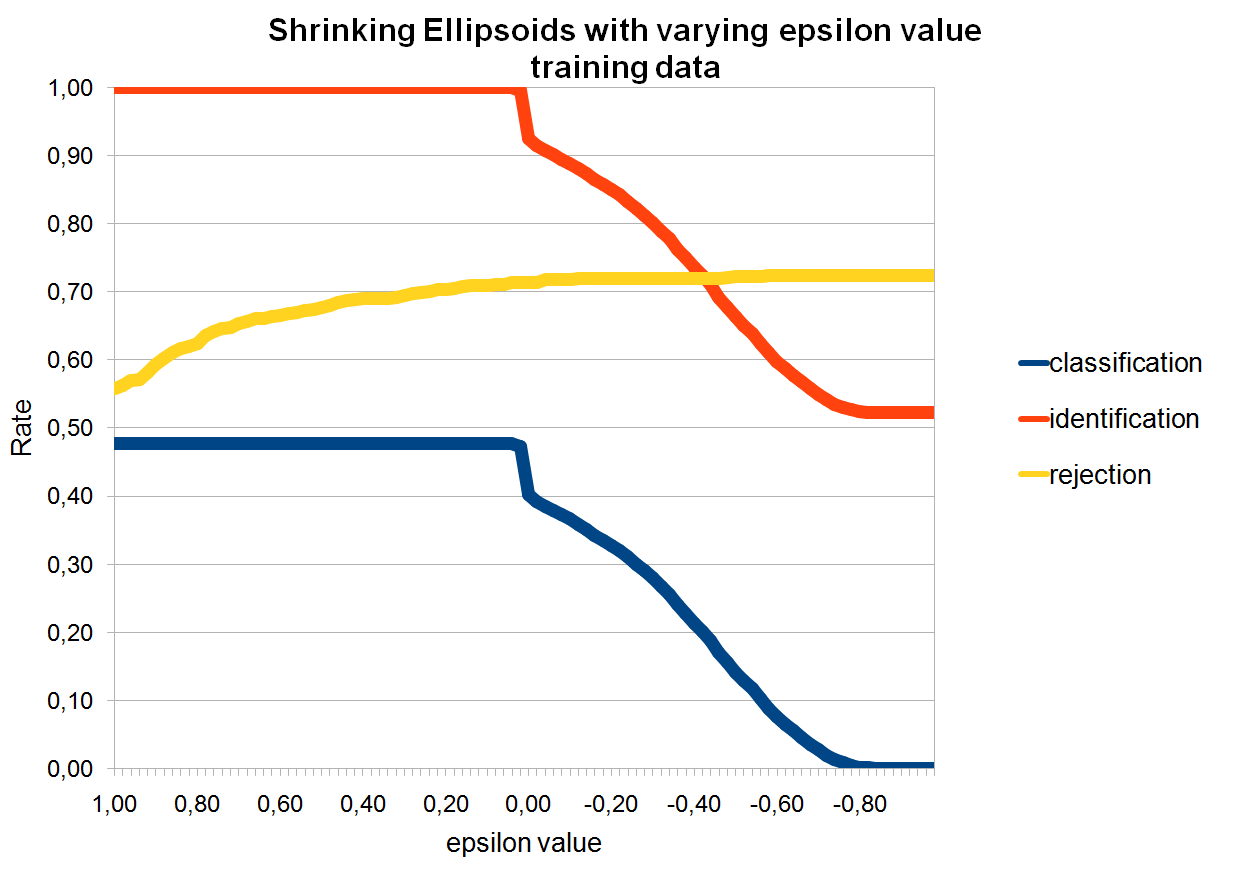
\includegraphics[width=0.80\textwidth]{Figures/charts/MUSIC_NOTES/DIGITS_ShrinkingEllipsoidsToleranceTraining.png}
	\hspace{12pt}
	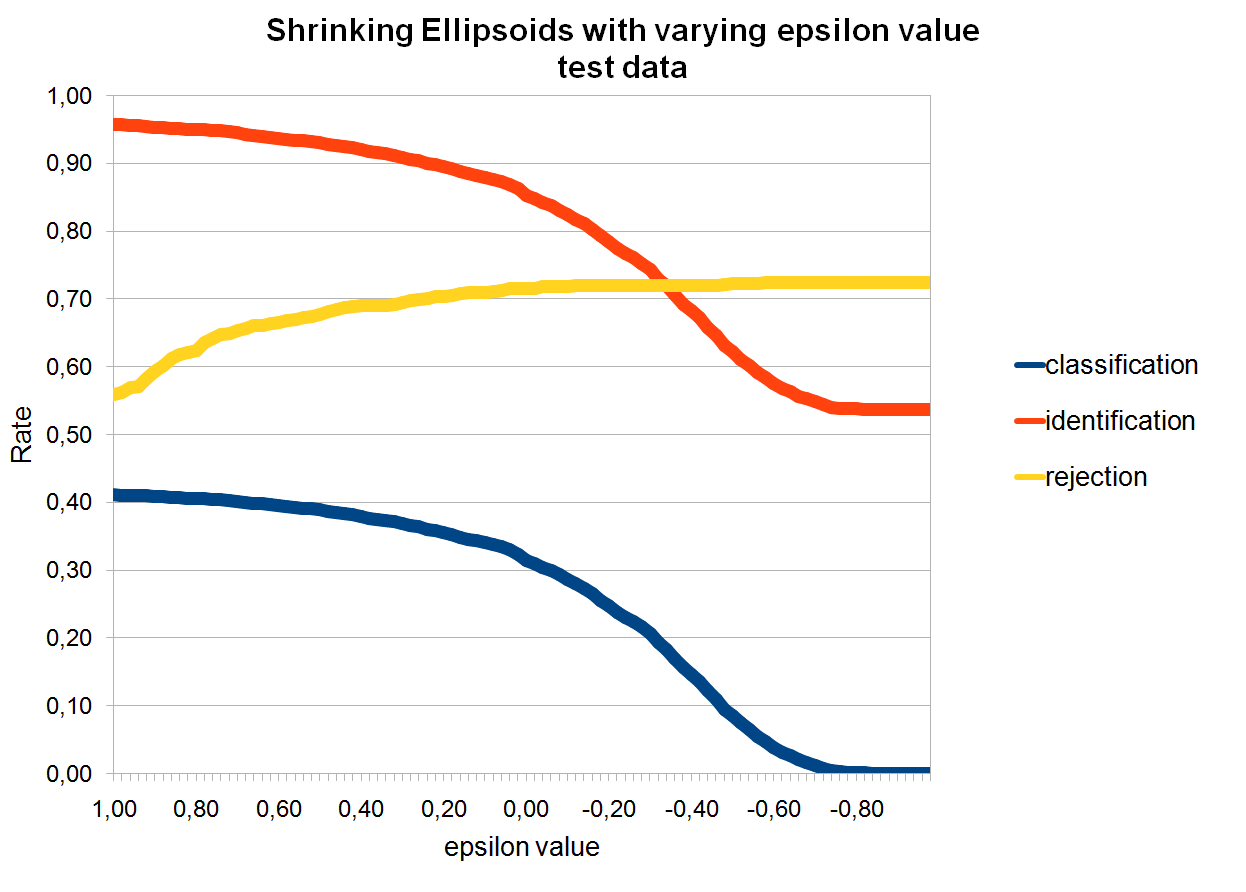
\includegraphics[width=0.80\textwidth]{Figures/charts/MUSIC_NOTES/DIGITS_ShrinkingEllipsoidsToleranceTest.png}
	\caption{ Identification, Classification and Rejection rates obtained for different $\varepsilon$ values, tested on training and test data consisting of 20 native classes and 1 foreign one, representing musical notes. Minimum volume enclosing figure is ellipsoid. }
	\label{fig:shrinking_music_notes}
\end{figure}

\begin{figure}[htp]
	\centering
	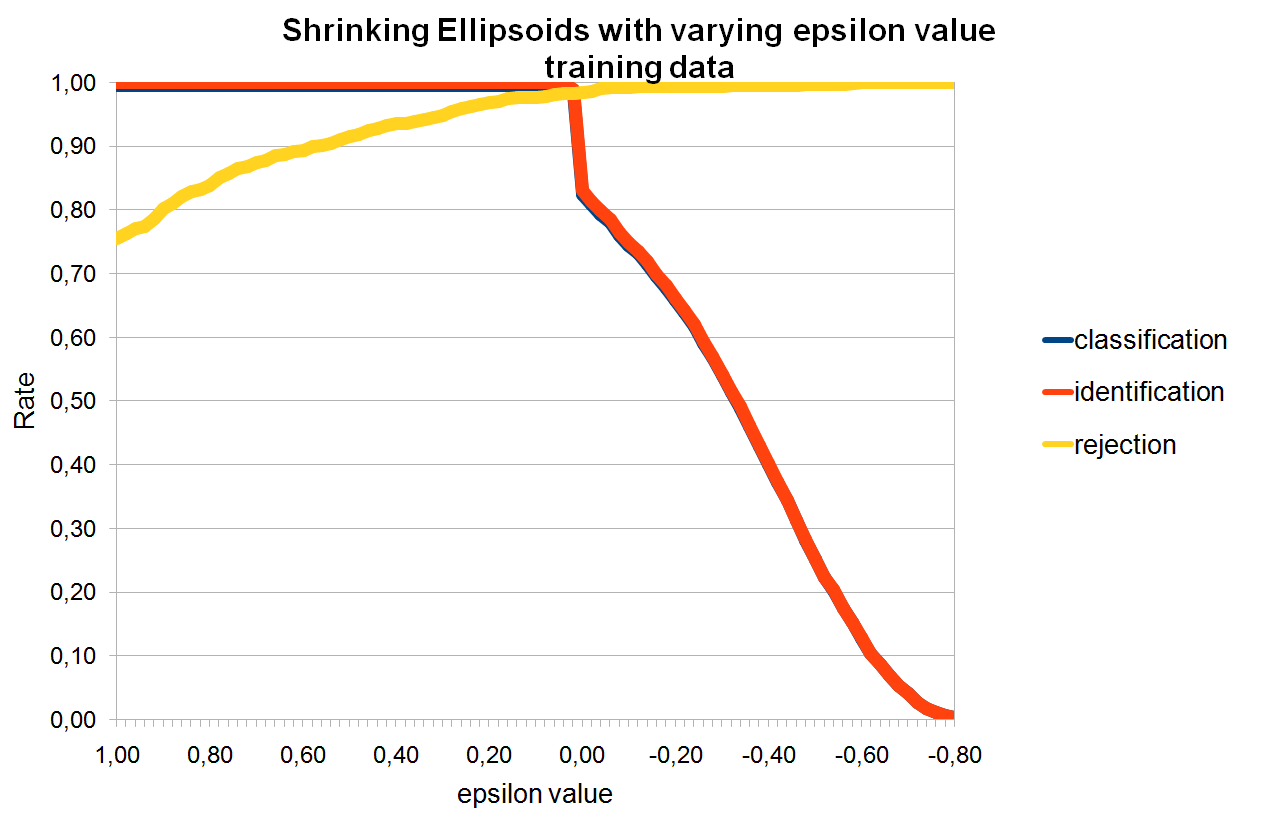
\includegraphics[width=0.80\textwidth]{Figures/charts/MUSIC_NOTES_STANDARIZED/DIGITS_ShrinkingEllipsoidsToleranceTraining.png}
	\hspace{12pt}
	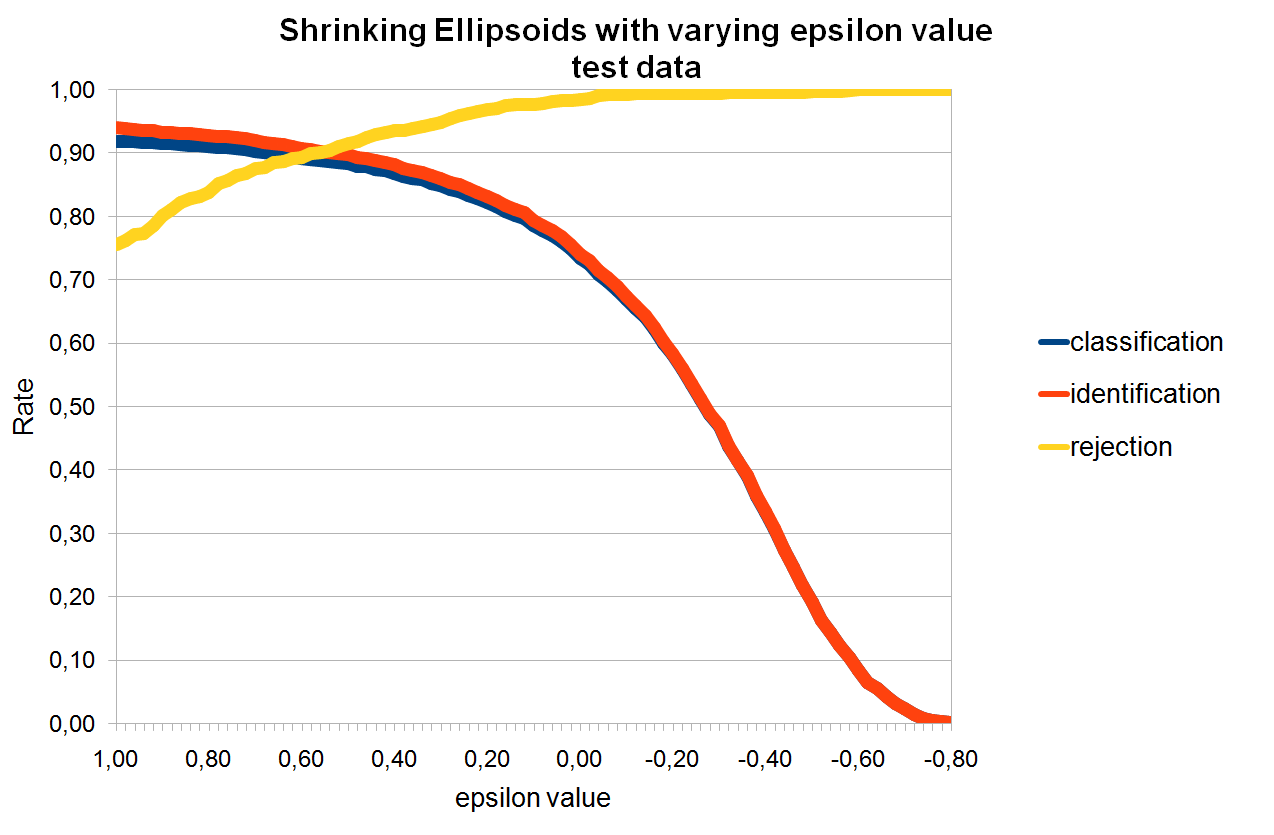
\includegraphics[width=0.80\textwidth]{Figures/charts/MUSIC_NOTES_STANDARIZED/DIGITS_ShrinkingEllipsoidsToleranceTest.png}
	\caption{ Identification, Classification and Rejection rates obtained for different $\varepsilon$ values, tested on training and test data consisting of 20 native classes and 1 foreign one, representing musical notes. Each feature from the feature vector has been standardized. Minimum volume enclosing figure is ellipsoid. }
\end{figure}

\begin{figure}[htp]
	\centering
	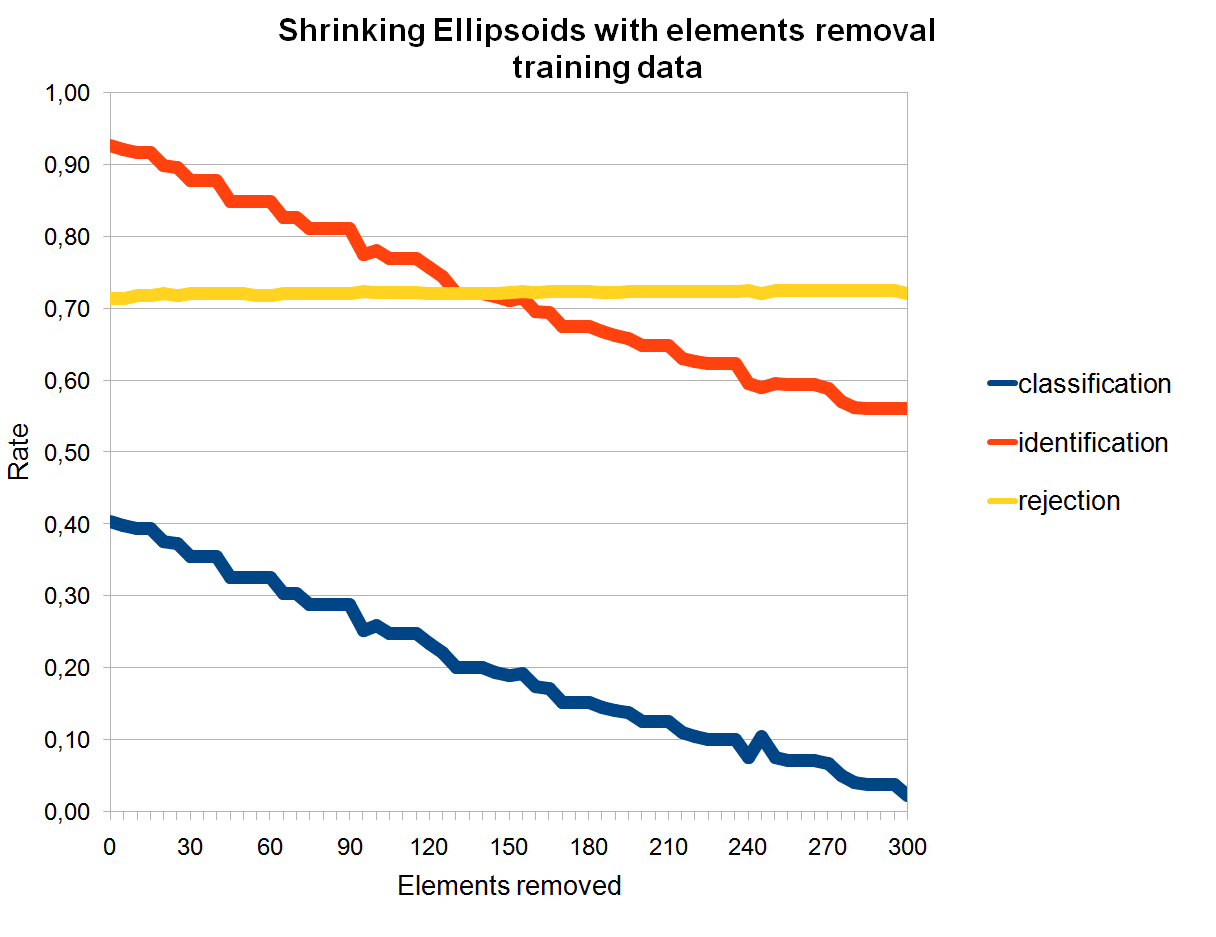
\includegraphics[width=0.80\textwidth]{Figures/charts/MUSIC_NOTES/DIGITS_ShrinkingEllipsoidsElementsRemovalTraining.png}
	\hspace{12pt}
	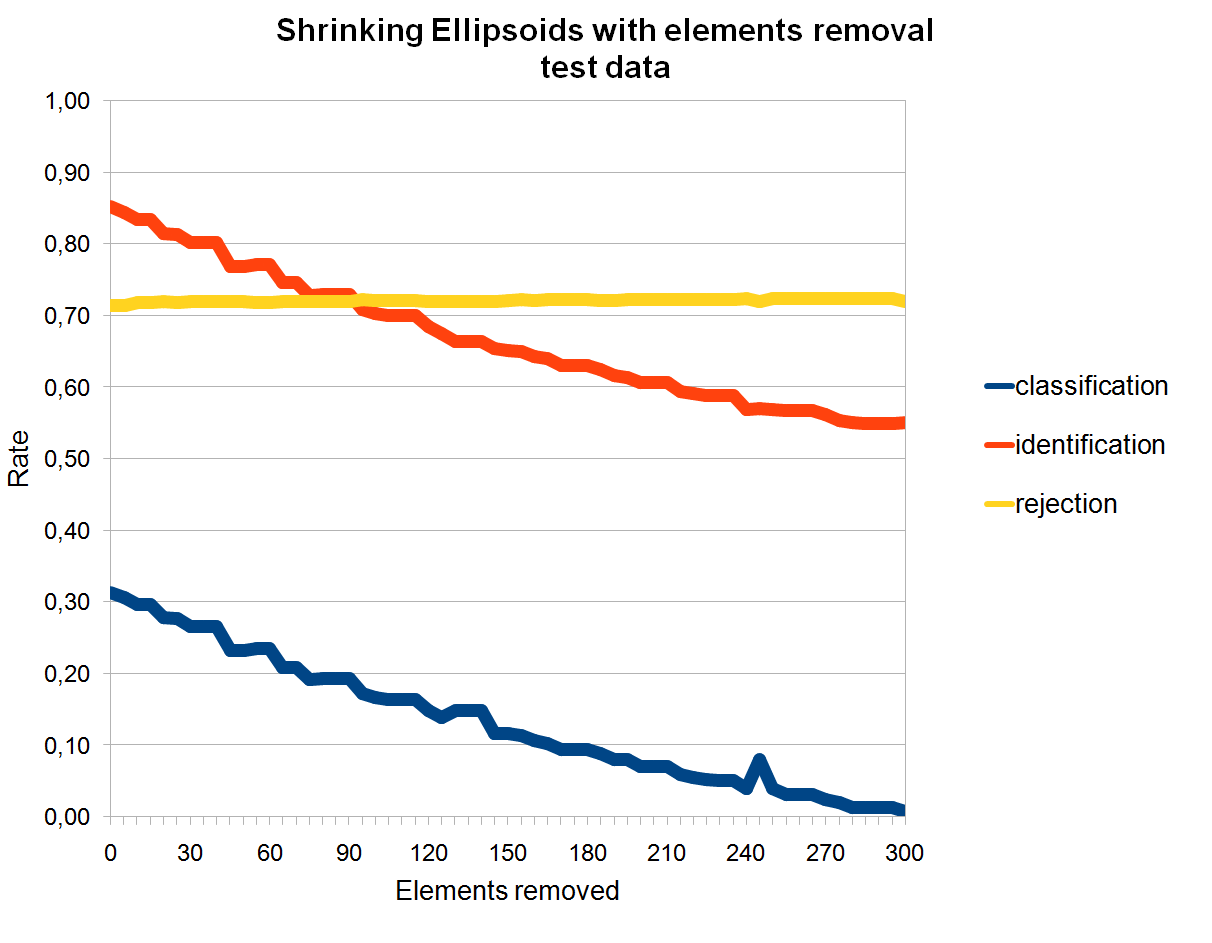
\includegraphics[width=0.80\textwidth]{Figures/charts/MUSIC_NOTES/DIGITS_ShrinkingEllipsoidsElementsRemovalTest.png}
	\caption{ Identification, Classification and Rejection rates obtained for increasingly smaller data sets, tested on training and test data consisting of 20 native classes and 1 foreign one, representing musical notes. Minimum volume enclosing figure is ellipsoid. }
\end{figure}

\begin{figure}[htp]
	\centering
	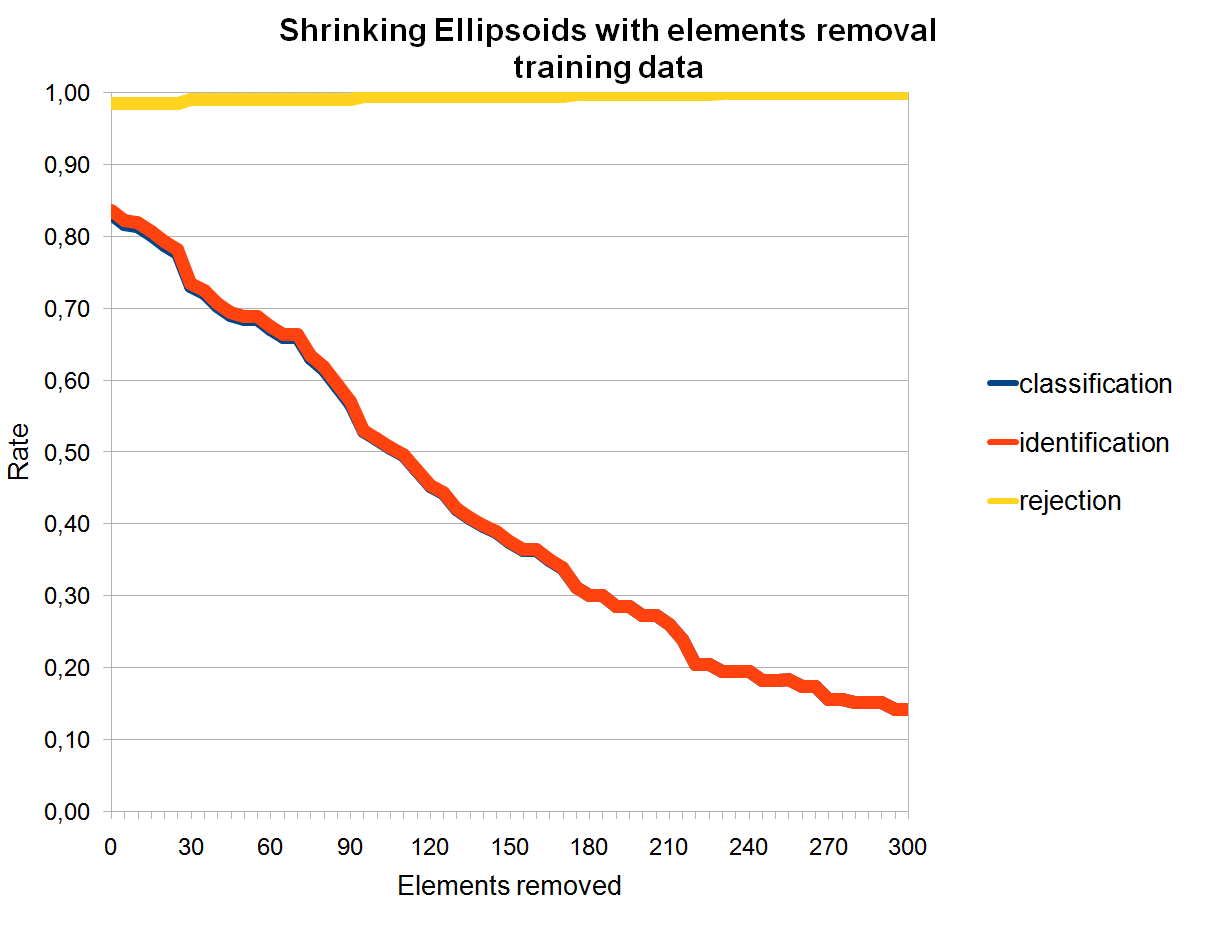
\includegraphics[width=0.80\textwidth]{Figures/charts/MUSIC_NOTES_STANDARIZED/DIGITS_ShrinkingEllipsoidsElementsRemovalTraining.png}
	\hspace{12pt}
	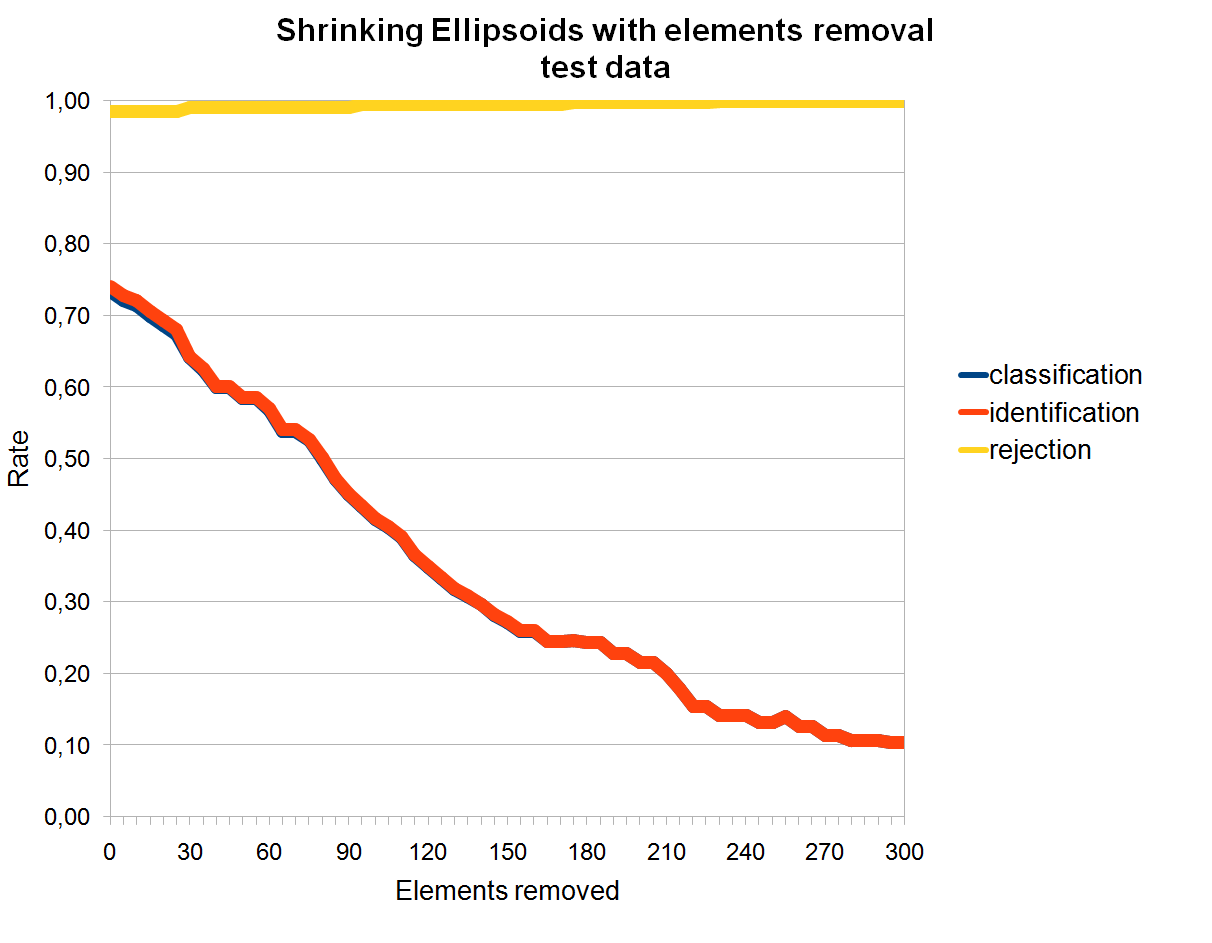
\includegraphics[width=0.80\textwidth]{Figures/charts/MUSIC_NOTES_STANDARIZED/DIGITS_ShrinkingEllipsoidsElementsRemovalTest.png}
	\caption{ Identification, Classification and Rejection rates obtained for increasingly smaller data sets, tested on training and test data consisting of 20 native classes and 1 foreign one, representing musical notes. Each feature from the feature vector has been standardized. Minimum volume enclosing figure is ellipsoid. }
\end{figure}


\begin{figure}[htp]
	\centering
	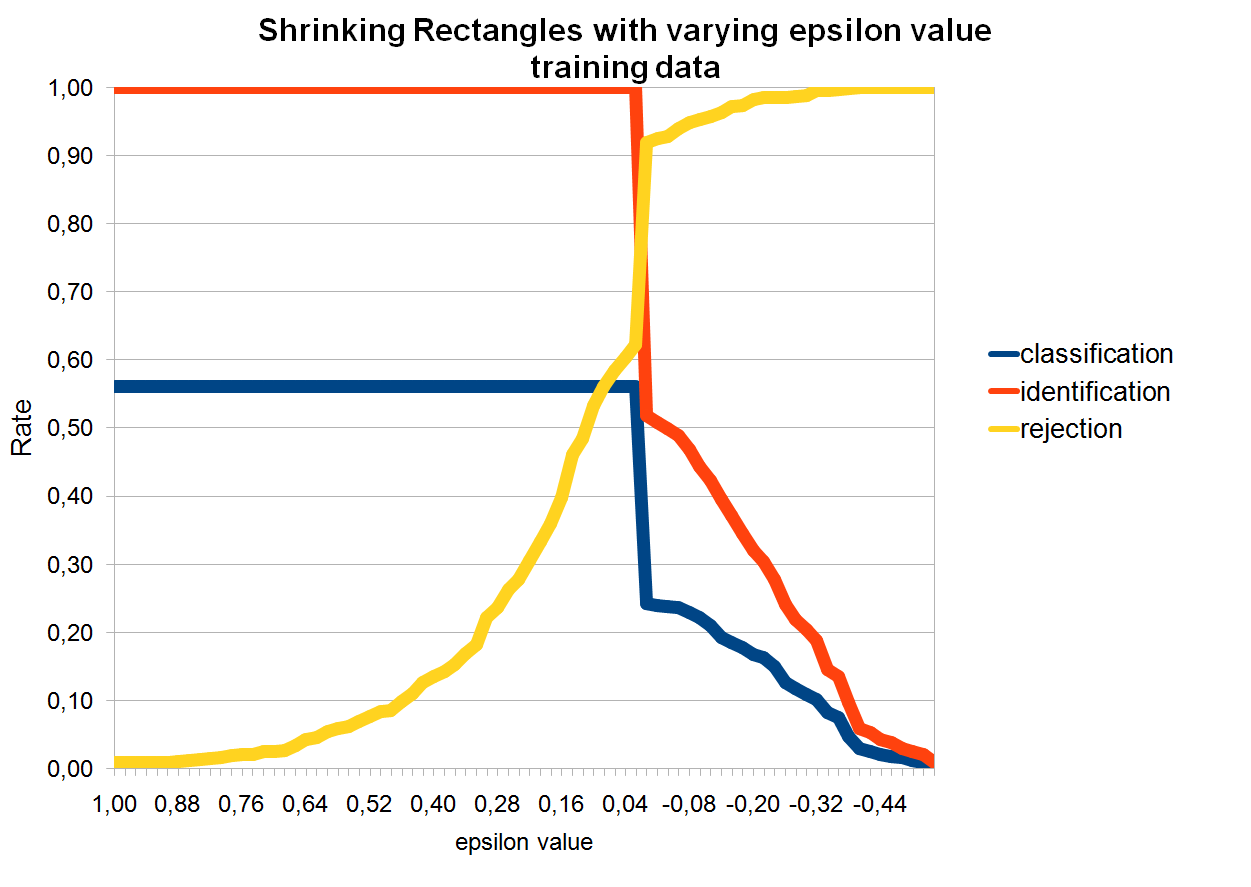
\includegraphics[width=0.80\textwidth]{Figures/charts/MUSIC_NOTES/DIGITS_ShrinkingRectanglesToleranceTraining.png}
	\hspace{12pt}
	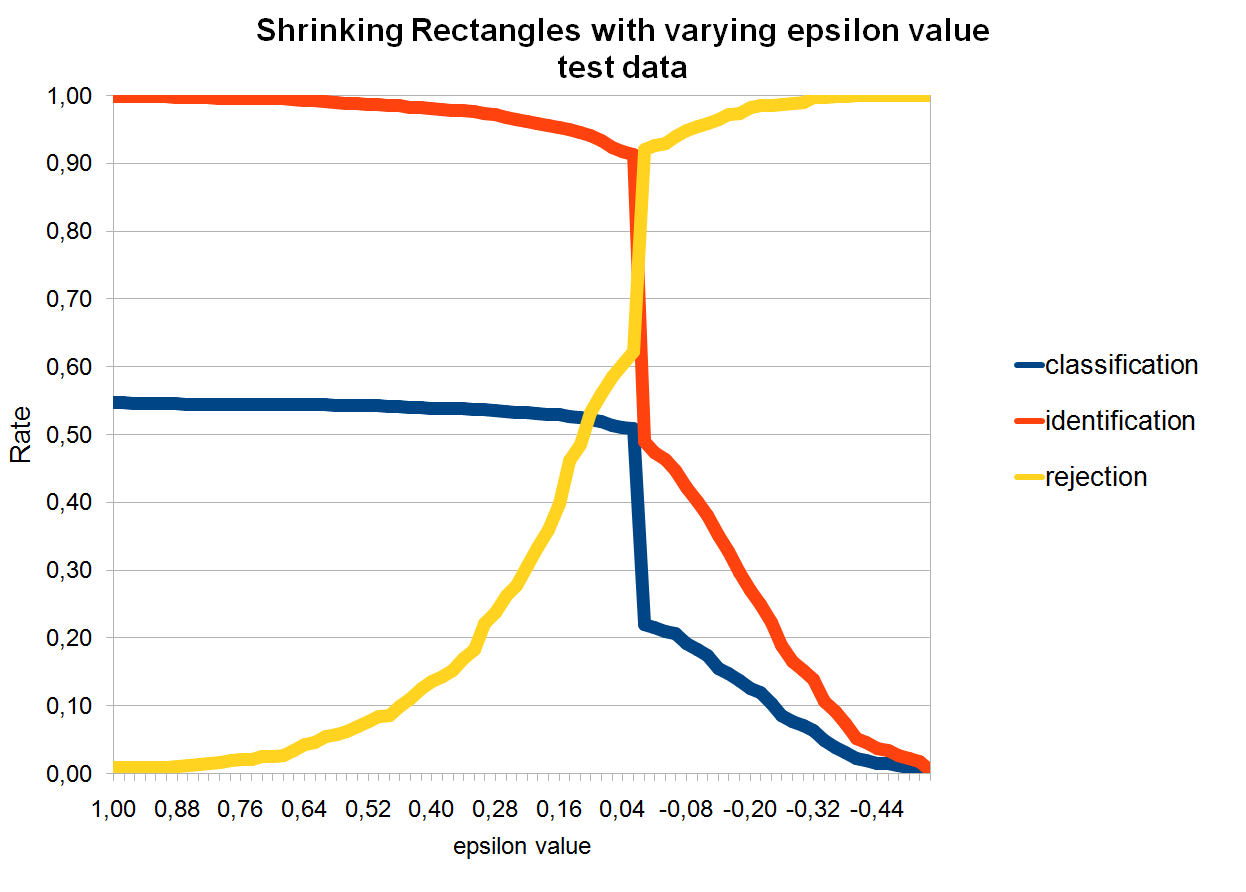
\includegraphics[width=0.80\textwidth]{Figures/charts/MUSIC_NOTES/DIGITS_ShrinkingRectanglesToleranceTest.png}
	\caption{ Identification, Classification and Rejection rates obtained for different $\varepsilon$ values, tested on training and test data consisting of 20 native classes and 1 foreign one, representing musical notes. Minimum volume enclosing figure is hyper rectangle. }
\end{figure}

\begin{figure}[htp]
	\centering
	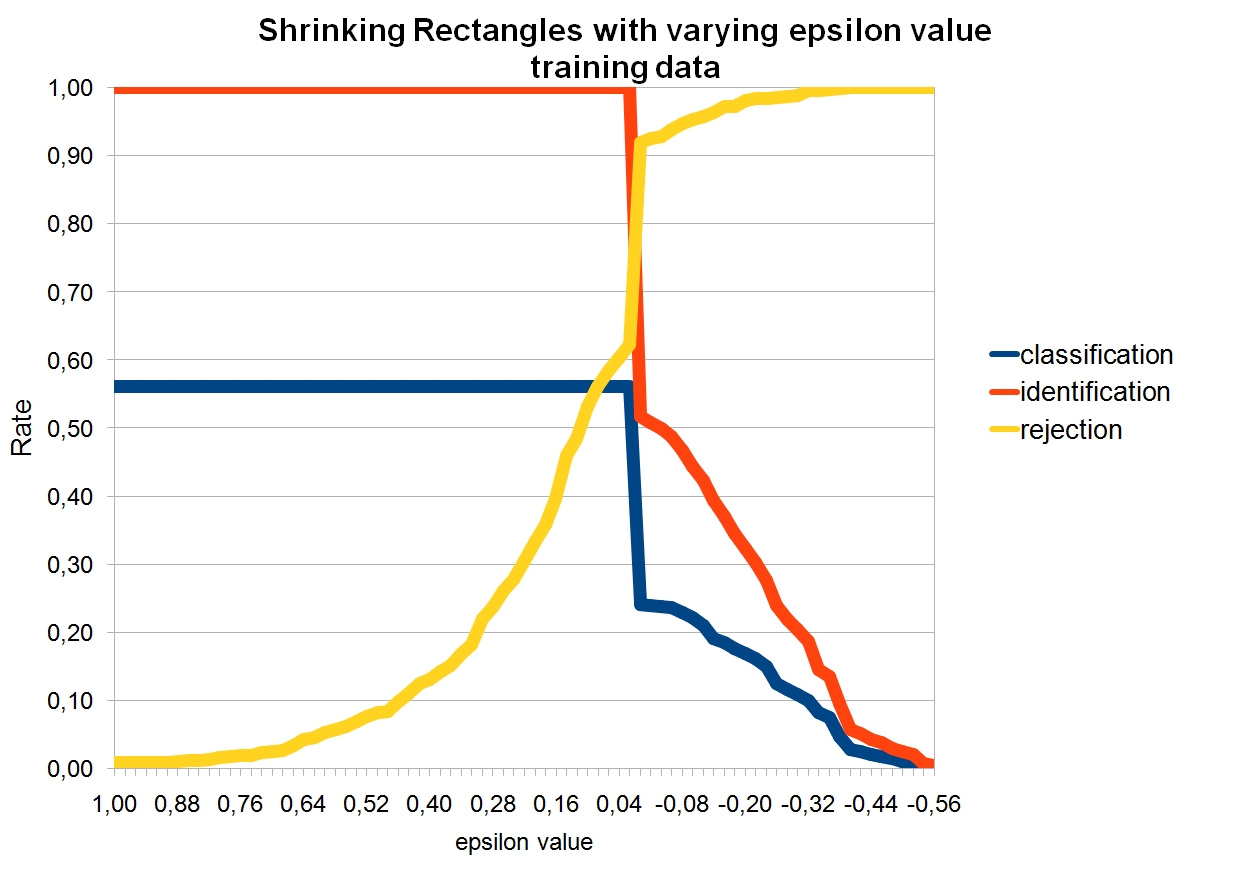
\includegraphics[width=0.80\textwidth]{Figures/charts/MUSIC_NOTES_STANDARIZED/DIGITS_ShrinkingRectanglesToleranceTraining.png}
	\hspace{12pt}
	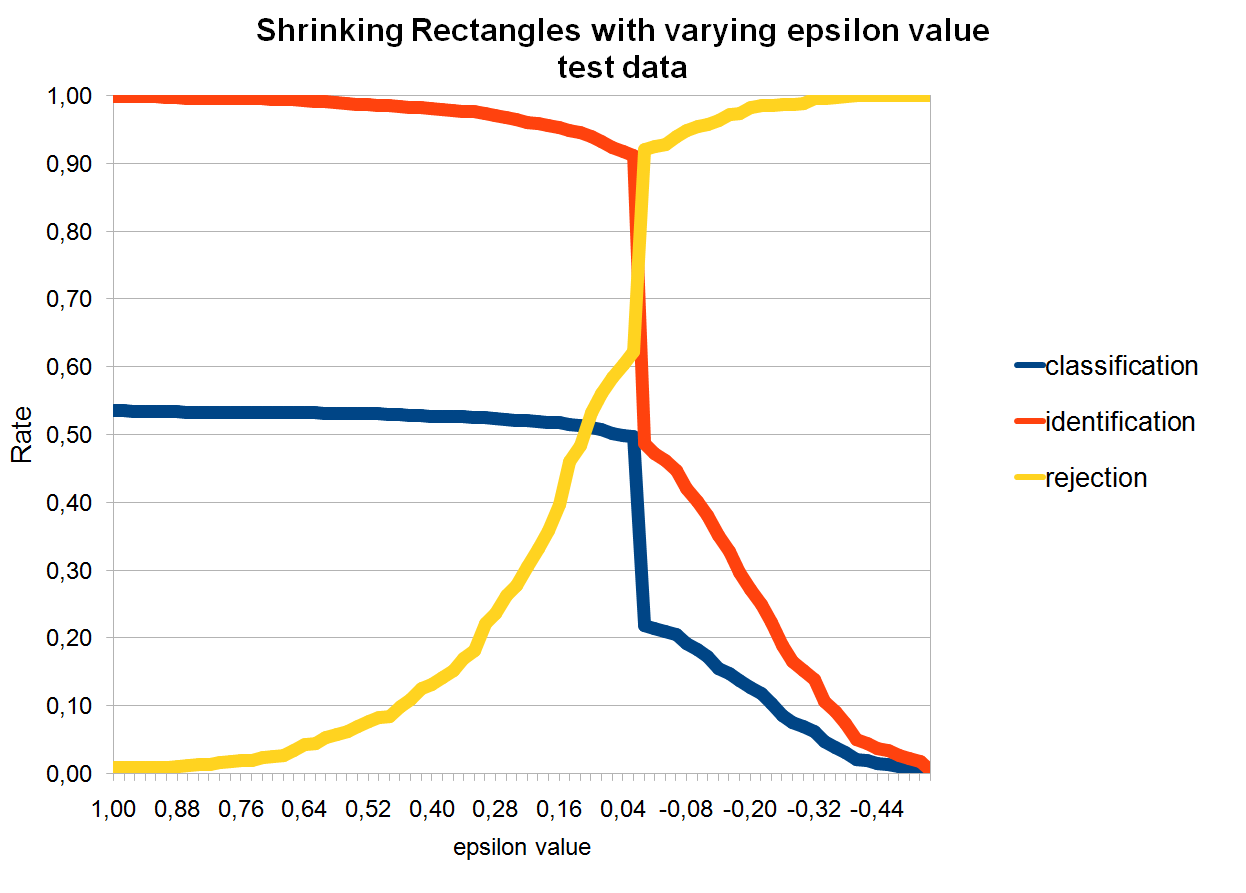
\includegraphics[width=0.80\textwidth]{Figures/charts/MUSIC_NOTES_STANDARIZED/DIGITS_ShrinkingRectanglesToleranceTest.png}
	\caption{ Identification, Classification and Rejection rates obtained for different $\varepsilon$ values, tested on training and test data consisting of 20 native classes and 1 foreign one, representing musical notes. Each feature from the feature vector has been standardized. Minimum volume enclosing figure is hyper rectangle. }
\end{figure}

\begin{figure}[htp]
	\centering
	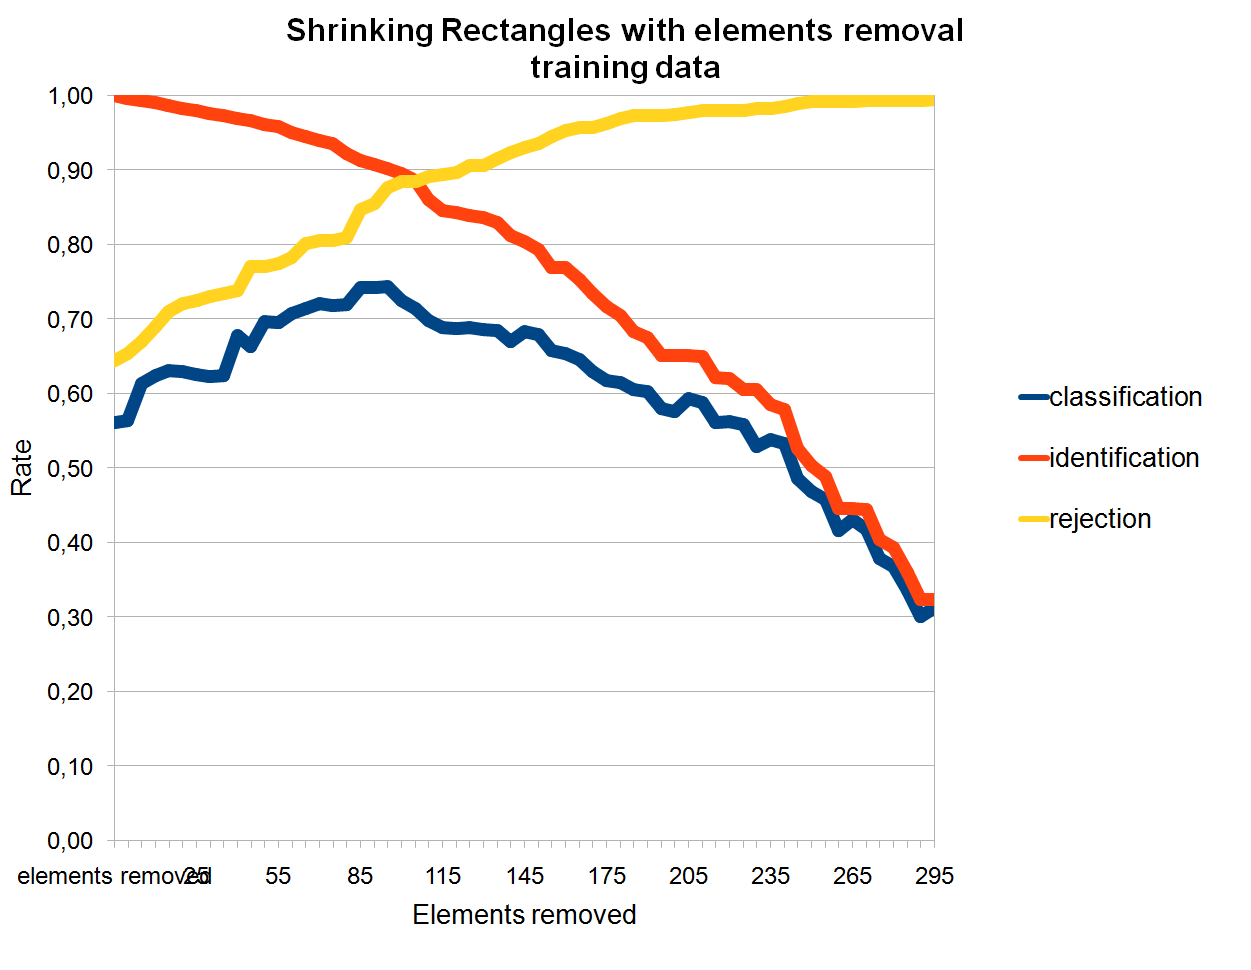
\includegraphics[width=0.80\textwidth]{Figures/charts/MUSIC_NOTES/DIGITS_ShrinkingRectanglesElementsRemovalTraining.png}
	\hspace{12pt}
	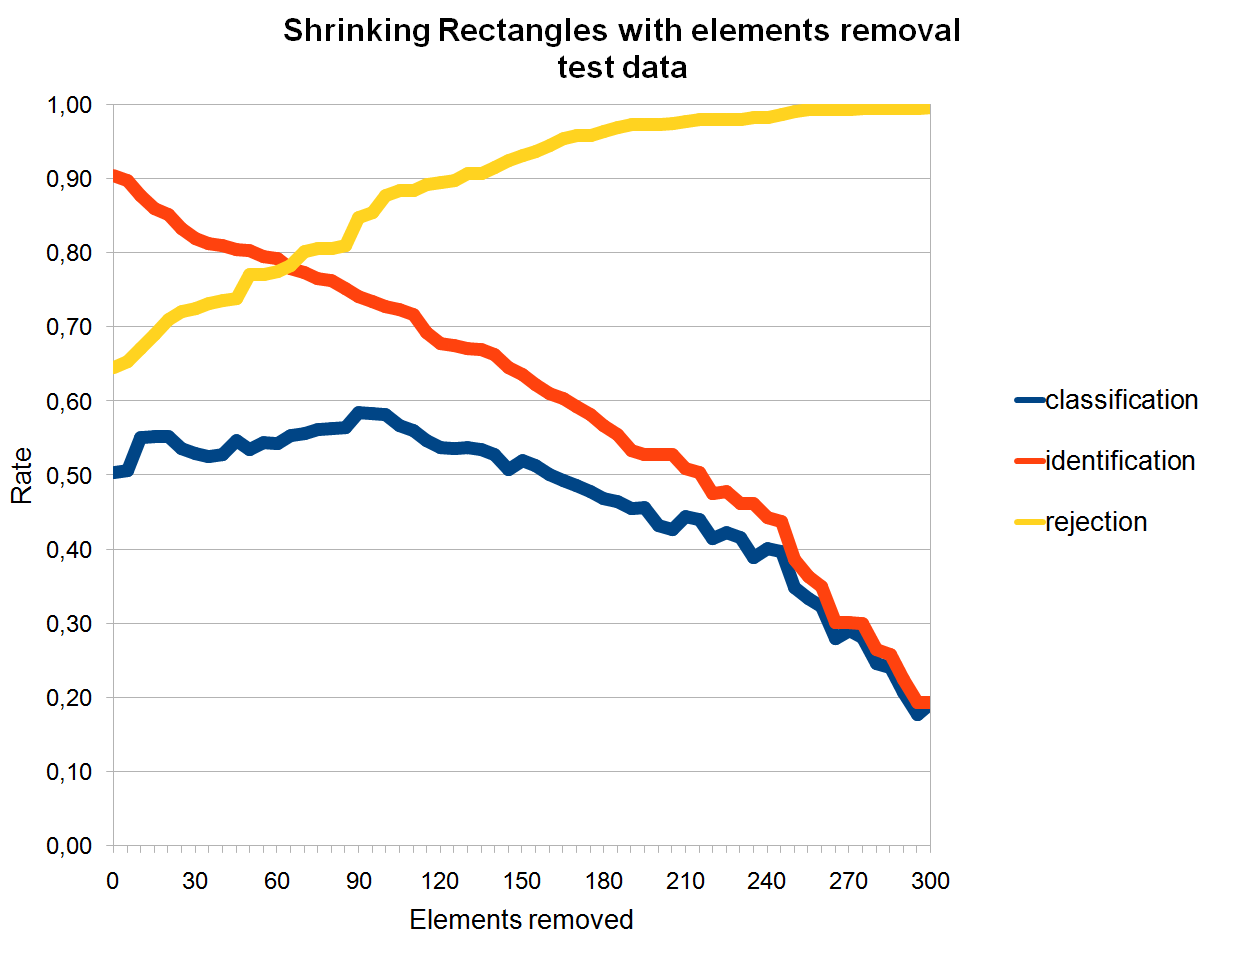
\includegraphics[width=0.80\textwidth]{Figures/charts/MUSIC_NOTES/DIGITS_ShrinkingRectanglesElementsRemovalTest.png}
	\caption{ Identification, Classification and Rejection rates obtained for increasingly smaller data sets, tested on training and test data consisting of 20 native classes and 1 foreign one, representing musical notes. Minimum volume enclosing figure is hyper rectangle. }
\end{figure}

\begin{figure}[htp]
	\centering
	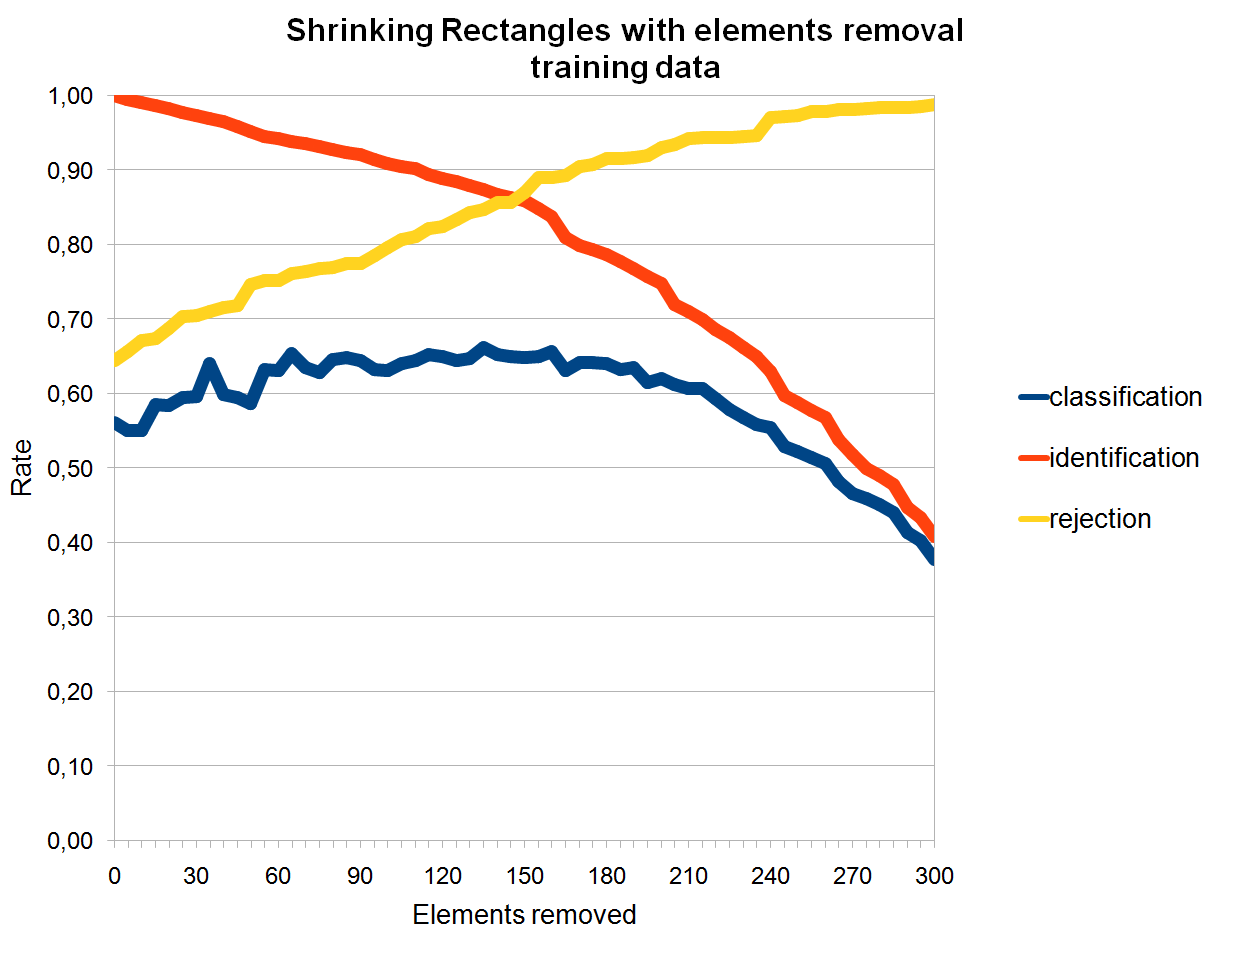
\includegraphics[width=0.80\textwidth]{Figures/charts/MUSIC_NOTES_STANDARIZED/DIGITS_ShrinkingRectanglesElementsRemovalTraining.png}
	\hspace{12pt}
	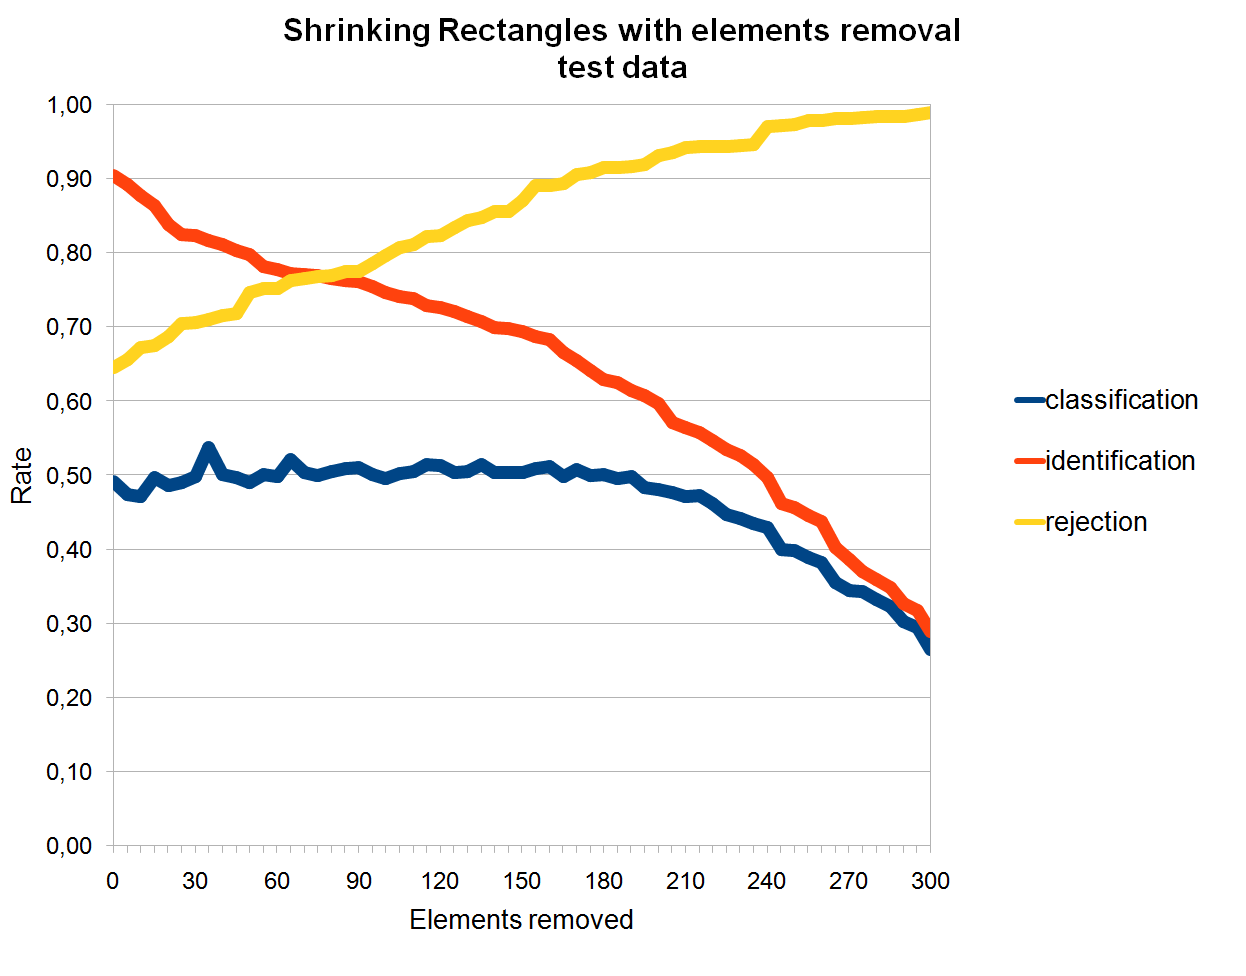
\includegraphics[width=0.80\textwidth]{Figures/charts/MUSIC_NOTES_STANDARIZED/DIGITS_ShrinkingRectanglesElementsRemovalTest.png}
	\caption{ Identification, Classification and Rejection rates obtained for increasingly smaller data sets, tested on training and test data consisting of 20 native classes and 1 foreign one, representing musical notes. Each feature from the feature vector has been standardized. Minimum volume enclosing figure is hyper rectangle. }
\end{figure}